\documentclass[9pt,a4paper]{article}
\usepackage[utf8]{inputenc}

\title{CSE 300: Online Assignment}
\author{Md Shamsuzzoha Bayzid$^{1,*}$, Mahjabin Nahar$^{1,\tau}$, Md Shariful Islam Bhuyan$^{1,\tau}$,\\
and Md Saidur Rahman$^{1,\tau}$\\ 
$^1$Department of Computer Science and Engineering\\
Bangladesh University of Engineering and Technology\\
$^*$Corresponding author: shams bayzid@cse.buet.ac.bd\\
$^\tau$These authors contributed equally to this work}
\date{\today}

%\usepackage{natbib} 

\usepackage{graphicx}
\usepackage{multirow}
\usepackage{multicol}
%\usepackage{biblatex}
\usepackage{enumerate}
\usepackage{float}
\usepackage{color}
\usepackage{amsfonts,amssymb,amsmath}



\begin{document}

\maketitle
%\tableofcontents
\section{Introduction}
This assignment has been designed to assess the preparation of the students in writing
scientific articles using \LaTeX\ . Different components, that are frequently used in scientific
manuscripts, have been covered in this assignment.

\subsection{Table}%\label{subsec:2.1}
We wish to place Table 1 right here.
\begin{table}[h]
    \centering
    \caption{\textbf{Optimization scores for Method-1 and Method-2 on different datasets
covering various model conditions.} We show average scores of two optimization
criteria for various model conditions.
}
    \begin{tabular}{|p{0.6in}|p{0.6in}p{0.6in}|p{0.6in}p{0.6in}|p{0.6in}p{0.6in}|}
\hline
\multicolumn{3}{|l|}{Simulation Condition}                               & \multicolumn{4}{l|}{Optimization Score}                   \\ \hline
\multirow{2}{*}{Dataset} & \multirow{2}{*}{Complexity} & Model Condition & \multicolumn{2}{l|}{Score1} & \multicolumn{2}{l|}{Score2} \\ \cline{4-7} 
                         &                             &                 & Method1      & Method2      & Method1      & Method2      \\ \hline
\end{tabular}
\begin{tabular}{|p{0.6in}|p{0.6in}p{0.6in}|p{0.6in}p{0.6in}|p{0.6in}p{0.6in}|}
\hline
\multirow{4}{*}{D1} & \multirow{2}{*}{Easy} & M1 & 7425.55 & 770.00  & 929.00  & 10 \\
                    &                       & M2 & 7657.66 & 9179.00 & 764.55  & 20 \\ \cline{2-7} 
                    & \multirow{2}{*}{Hard} & M3 & 54.00   & 9007.00 & 3759.00 & 30 \\
                    &                       & M4 & 74.00   & 5567.00 & 99.00   & 25 \\ \hline
\end{tabular}
\begin{tabular}{|p{0.6in}|p{0.6in}p{0.6in}|p{0.6in}p{0.6in}|p{0.6in}p{0.6in}|}
\hline
\multirow{3}{*}{D2} & \multirow{3}{*}{Moderate} & M1 & 34.00            & 273.00           & 321.60 & 34 \\
                    &                           & M2 & \multicolumn{2}{l|}{Not Applicable} & 16.00  & 11 \\
                    &                           & M3 & 657.00           & 179.00           & 716.00 & 19 \\ \hline
\end{tabular}
    
    %\label{tab:my_label}
\end{table}
\newpage
\begin{figure}[h]
	\centering
	%\caption{This caption is at the top}
	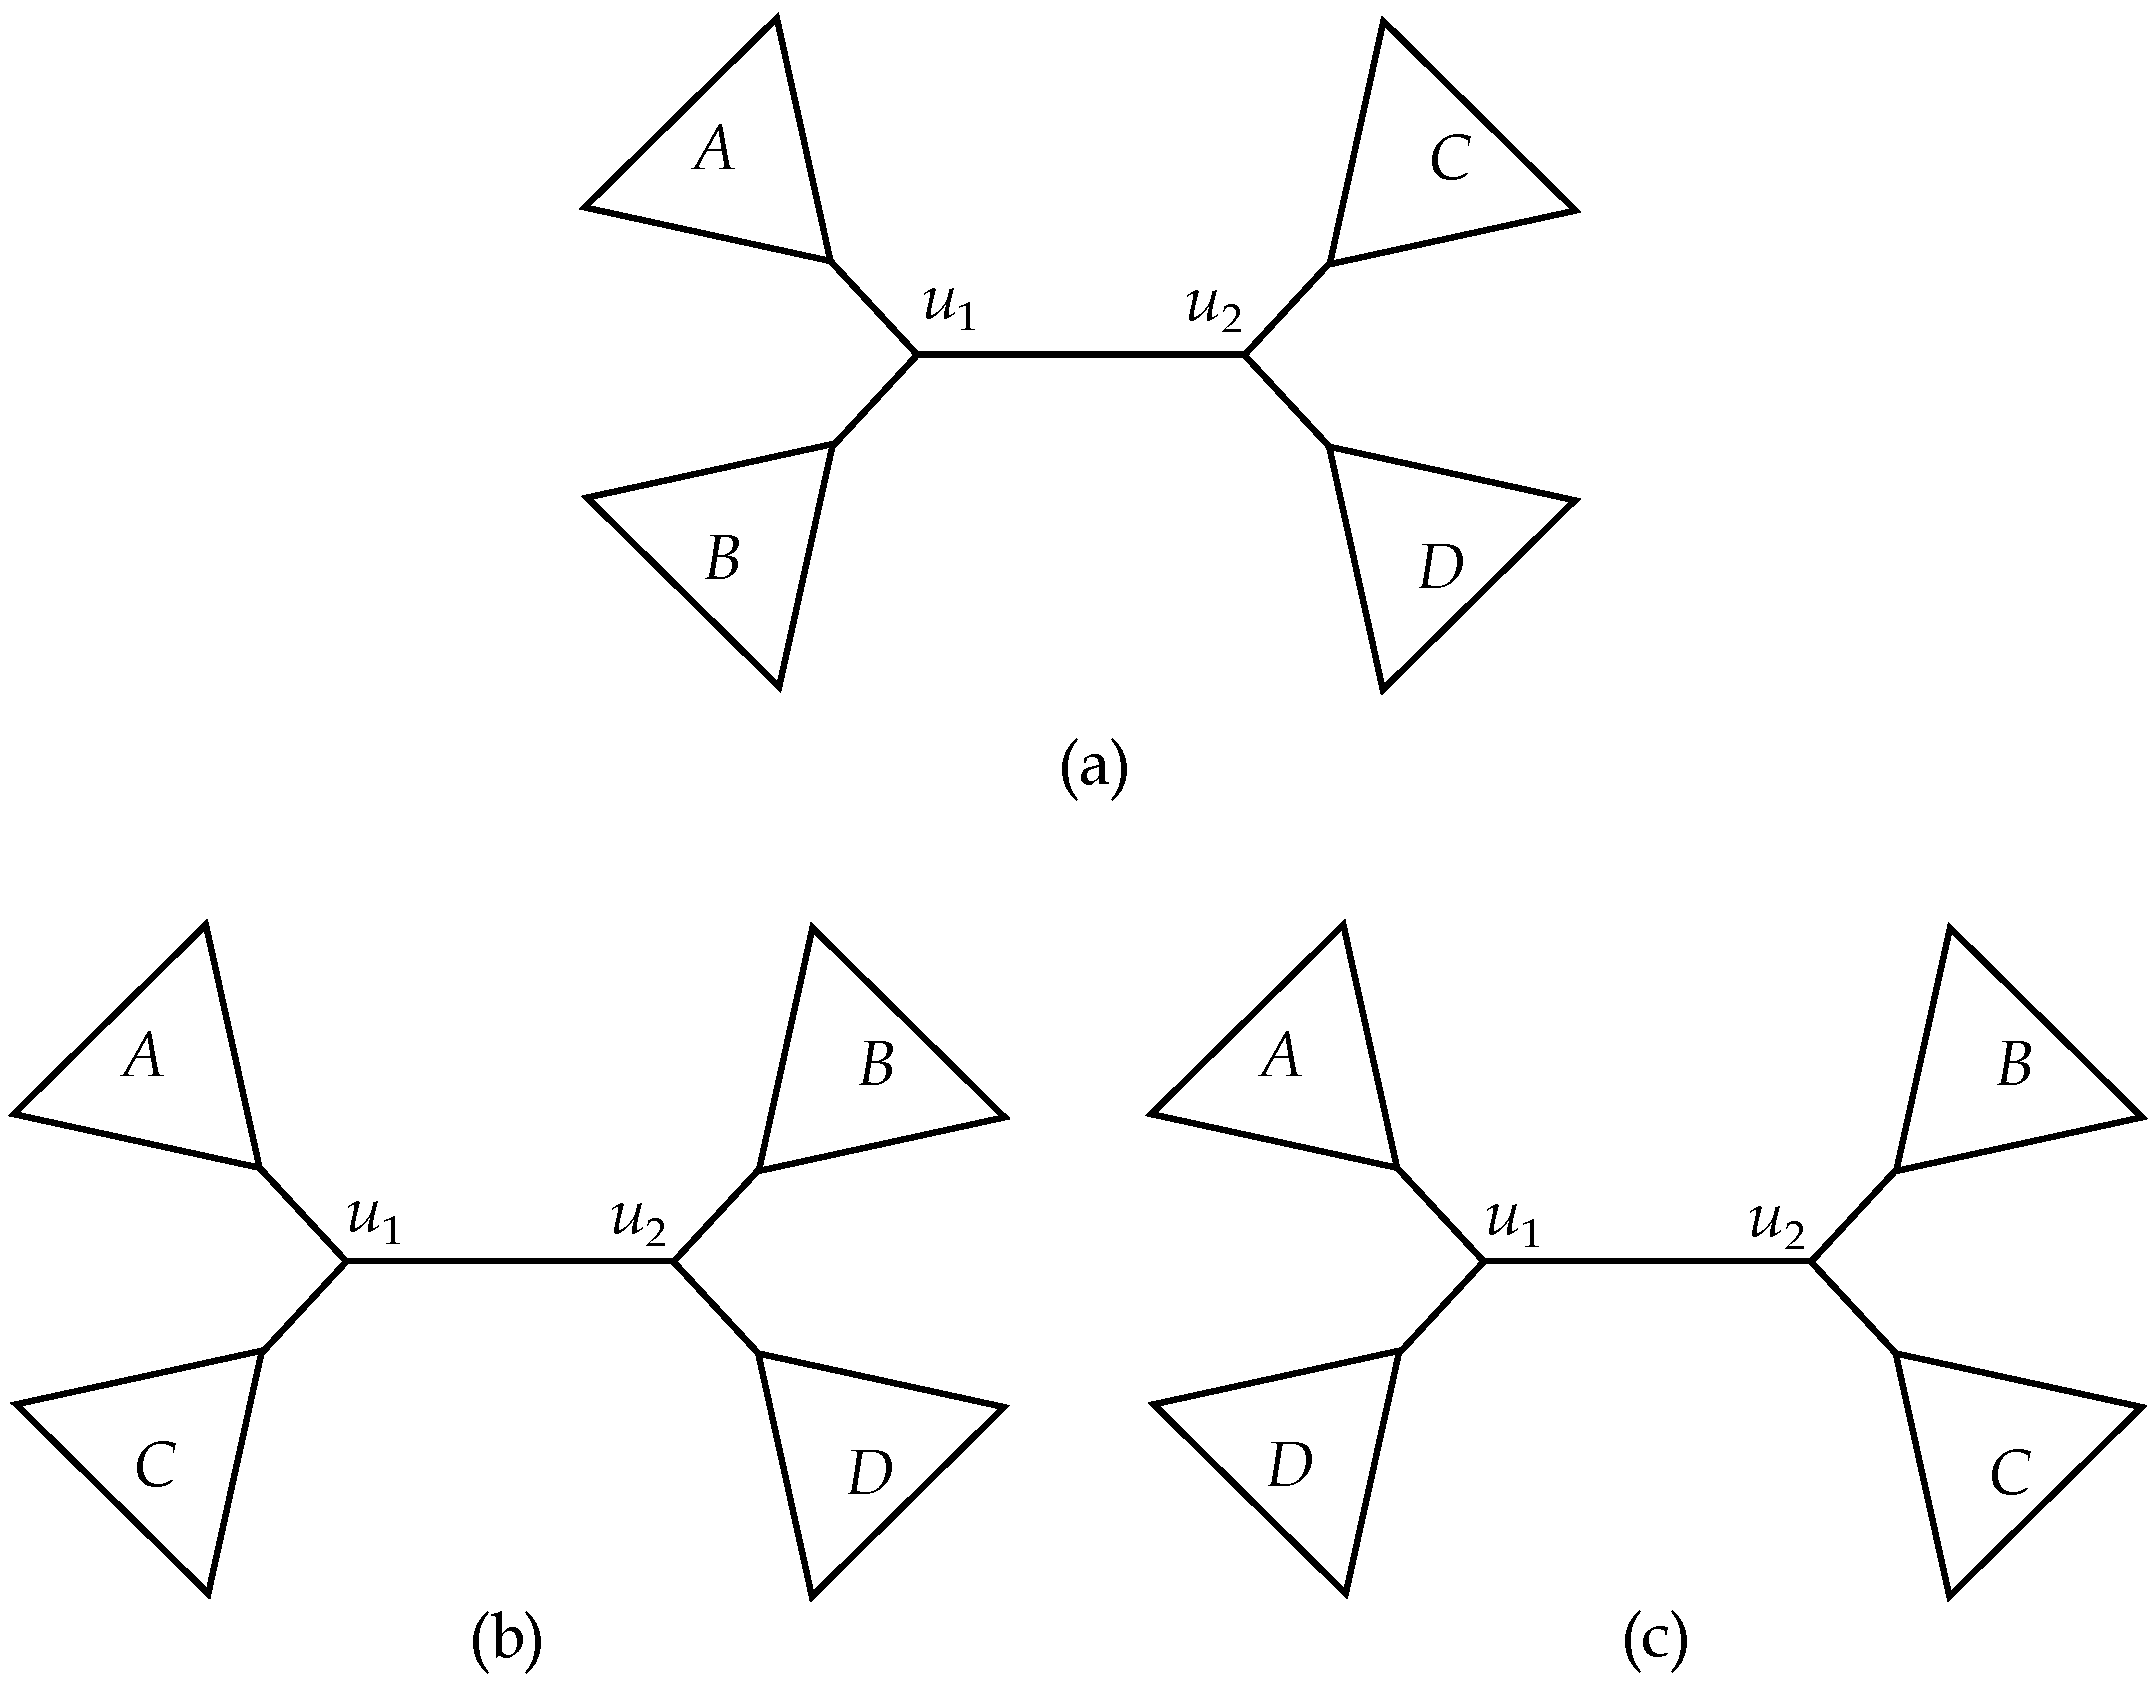
\includegraphics[scale=0.4]{Figure3.pdf}
	%\label{fig:1}
	\caption{\textbf{Nearest Neighbor Interchange (NNI) move on an internal edge.} (a)
A species tree $ST$, and (b)-(c) the neighbors of $ST$ resulting from one NNI move on edge
$e = (u1, u2). A, B, C$, and $D$ are the sets of taxa in the four subtrees around edge $e$}
\end{figure}
\subsection{Figures}
We intend to put Figure 1 at the top of a page.
\subsection{Equations}
Let n1|n2|n3 be a tripartition defined on an internal node u of a binary tree T. The number of tripartitions mapped to u is given by Eqn. 1.
\begin{equation}
 NQ(n1,n2,n3) = \left (n1 \atop 2 \right )\left (n2 \atop 1 \right )\left (n3 \atop 1 \right ) +  \left (n2 \atop 2 \right )\left (n1 \atop 1 \right )\left (n3 \atop 1 \right ) +  \left (n3 \atop 2 \right )\left (n1 \atop 1 \right )\left (n2 \atop 1 \right )\\ 
 = \frac{n1n2n3(n1+n2+n3-3)}{2}
\end{equation}  
\section{Conclusion}
The major objectives of this assignment are listed below ( please do notignore the font
sizes).
\begin{enumerate}[\textbullet] %if we want to start from anything :\setcounter{enumi}{5}
    \item \begin{Large}{To assess the ability of the students in preparing manuscripts
in} \LaTeX\ .\end{Large}
\newpage
     \item \begin{large}{To assess the ability of the students in preparing manuscripts
in} \LaTeX\ .\end{large}
\item \begin{normalsize}{To assess the ability of the students in preparing manuscripts
in} \LaTeX\ .\end{normalsize} 
 \item \begin{footnotesize}{To assess the ability of the students in preparing manuscripts
in} \LaTeX\ .\end{footnotesize}



\end{enumerate}



























\end{document}
